\documentclass[a4paper,11pt]{article}

\usepackage[margin=2.5cm]{geometry}
\usepackage{booktabs} 
\usepackage{amsmath}
\usepackage{amssymb}
\usepackage{graphicx}
\usepackage{caption}
\usepackage{natbib}
\usepackage{xcolor}

\newcommand{\p}{\partial}
\newcommand{\gzm}{{\xi}}%{\gamma z_\text{match}}}
\newcommand{\todo}[1]{\textcolor{red}{$[$#1$]$}}

\pdfsuppresswarningpagegroup=1

\author{hauke-zrick}

\date{Draft \today}
\title{Towards a Universal Veering Profile for Turbulent Ekman Flow at arbitrary Reynolds number - Part 2\\
  \normalsize LES and DNS of Turbulent Ekman Flow \\}

\begin{document} 

\maketitle

\begin{abstract}
  An analytical formulation for the profiles of stream- and span-wise velocity in turbulent Ekman flow and large-eddy simulations are used to analyze the properties of the turbulent Ekman flow. 
%
	We show a comparison of a turbulent Ekman flow of $Re_D=1\,600$ simulated by DNS and LES.
\end{abstract}
%
%%%%%%%%%%%%%%%%%%%%%%%%%%%%%%%%%%%%%%%%%%%%%%%%%%%%%%%%%%%%%%%%%%%%%%%%%%%%%%%%
%
\section{Introduction}

We here consider the turbulent Ekman flow as a homogeneous, stationary boundary layer flow over a rotating flat surface under neutral stratification. This flow is defined by only very few parameters. Nevertheless, it can serve as a simple model of the atmospheric boundary layer since it exhibits many characteristics that also shape the real atmosphere, namely the logarithmic layer and the Ekman spiral. Hence, the investigation of this case is suited to learn about the fundamental properties of the atmospheric boundary layer.

We investigate three different Reynolds numbers $Re_D$: $1\,600$, 150\,000, and 1\,000\,000, where $Re_D = GD/\nu$ and $D=\sqrt{2\nu/f}$, $Re_D = G/\sqrt{\frac{1}{2}\nu f}$. All cases are simulated by LES and the low Reynolds number case we also compare to DNS for comparison. The too high Reynolds number cases cannot be simulated by DNS due to the limitations of computational resources.

Short summary of part I? In part I of this publication, we presented a generic profile of wind direction and speed in turbulent Ekman flow. 

The information how the wind direction changes with height is of great importance for wind-power forecasting \cite{optis2014moving}.

\todo{Wie ist die Grenzschicht? Was sagen die Profile und das LES darüber?}

Foundations: \cite{csanady1967resistance}, \cite{tennekes1973logarithmic}, \cite{spalart1989theoretical}

Neutral Ekman layer with LES: \cite{esau2004simulation}\cite{jiang2018large}

The same turbulent Ekman flow is simulated by DNS and LES and the results are compared. 

Profile of wind direction from DNS - what can be learned from it for LES?

Limits of coarse resolution

The velocity profiles of both horizontal components of the turbulent Ekman flow provide a benchmark test for LES model. $\rightarrow$ First step towards a generic wind profile including stratification (and inversion?)?

This paper investigates the mean velocity profiles of the turbulent Ekman flow from moderate to high Reynolds numbers using the formulation from part I and LES.

\section{A Universal Velocity Profile for the Turbulent Ekman Layer}

The universal velocity profile for the turbulent Ekman layer consists of several parts for different layers of the boundary layer. Near the surface, viscous forces dominate the flow. In the middle part, the velocity profile has a logarithmic shape which passes over into an Ekman spiral. 
In the following, the distinct layers for both horizontal components of the velocity are described.

\subsection{Total profile}

\todo{In part II a summary of the theor. profile in minimalistic form? Without any deductions, just a description.} 

From the layers of the velocity profile, a total profile for the whole boundary layer is formed. The profile of the stream-wise component of the velocity is seperated into three layers, which are the viscous layer $U_{visc}$, the logarithmic layer $U_{log}$, and the Ekman layer $U_{EK}$. The span-wise component of the velocity is seperated into two layers, namely the inner layer $V_{inner}$, and the Ekman layer $V_{EK}$.
\begin{align}
  U =& (1-w_{visc})U_{visc} + (w_{visc}-w_{outer})U_{log} + w_{outer}U_{EK}, \\
	V =& (1-w_{outer})V_{inner} + w_{outer}V_{EK}.
\end{align}
The transition between consecutive layers is formed by a transfer function:
\begin{align}\label{error}
  w_{*} = \frac{1}{2}\left(\textrm{erf}\left[\sigma_T\log\left(\frac{z}{z_{T}}\right)\right]+1\right),
\end{align}
where $\sigma_T$ is a transition scale that defines the width of the transition and $z_{T}$ is the height of the transition, where the upper and the lower layer equally contribute to the velocity ($w_{*}(z_{T})=0.5$).

\subsection{Drag-Law}

The geostrophic drag $Z \equiv u_\star/G$ and the direction between the shear stress and the geostrophic wind $\alpha$ are two key parameters of the Ekman flow. They can be estimated using a semi-empirical drag-law based on \cite{spalart1989theoretical}, which describes them as functions of only the Reynolds number:
\begin{subequations}\label{drag}
	\begin{align}
		\frac{G}{u_\star}\cos\phi^\star &= \frac{1}{\kappa}\log Re_\tau + C - A_r, \\
		\sin\phi^\star &= A_i\frac{u_\star}{G},\\
		\alpha &= \phi^\star - \frac{C_5}{Re_\tau},
	\end{align}
\end{subequations}
with $Re_\tau = \frac{Re_D^2}{2}\frac{u_\star^2}{G^2}$, $\kappa = 0.415$, $A_r = 4.80$, $A_i = -5.57$, $C = 5.4605$, $C_5 = -57.8$. This law is in excellent agreement with DNS in the range $400\leq Re_D\leq 1\,600$ as demonstrated by \cite{ansorge2014global}.

\subsection{Stream-wise Velocity Component}

In the viscous sublayer, the span-wise velocity is close to zero and the stream-wise velocity is described by the law of the wall:

\begin{align}
  U^{\alpha+} = z^+,
\end{align}
(the index $\alpha$ indicates the alignment with the direction of the shear stress). Around $z^+=5$, the velocity is beginning to deviate from its linear profile and the buffer layer forms the transition between viscous layer and logarithmic layer. From the surface up to the buffer layer, the stream-wise velocity is described by
\begin{align}
  U_{inner}^{\alpha+} = \frac{z^+ + \gamma_4(z^+)^4 + \gamma_6(z^+)^6}{1+\gamma_6/u_{ref}(z^+)^6},
\end{align}
where $\gamma_4=-3.825\cdot10^{-4}$, $\gamma_6=6.32\cdot10^{-6}$, and $u_{ref}=0.07825$.

The logarithmic region of the stream-wise velocity is 
\begin{align}
  U_{\log}^{\alpha+} = \frac{1}{\kappa}\log z^+ + C,
\end{align}
where $\kappa=0.416$, and $C=5.4605$. The transition between buffer layer and logarithmic layer is located at $z_T^+=19$ with a scale $\sigma_T=2$.

\subsection{Profile in Outer Layer}

Above the boundary layer, the horizontal pressure gradient is balanced by the coriolis force and the wind speed equals the geostrophic wind $G$. For the stationary case, the horizontal equations of motion can be written
\begin{subequations}
  \begin{align}
    0&=fV+\nu_e\partial_z^2U,\\
		0&=-f(U-G)+\nu_e\partial_z^2V,
  \end{align}
\end{subequations}
where $\nu_e$ is an eddy viscosity and the x-axis is aligned with the geostrophic wind. This is solved by
\begin{subequations}
  \begin{align}
    U_{EK} &= G + Ae^{-\tilde{z}}\cos\tilde{z},\\
		V_{EK} &= - Ae^{-\tilde{z}}\sin\tilde{z},
  \end{align}
\end{subequations}
where $A = 8.4u_\star - 150/Re_\tau$, $\tilde{z} = (z-z_r)/D_E$, $z_r = 0.12\delta$, and $D_E = 3\delta/4\pi\approx 0.24\delta$. The parameters are deduced from DNS.

The transition from the logarithmic layer to the Ekman layer is located at $z^-=0.3$ (talk: $z^-_T=0.3-120/Re_D$) with a transition scale of $\sigma_T=2$ for the stream-wise velocity.

\subsection{Span-wise Velocity}

For $z^+\leq10$, the knowledge on $U^\alpha$ is exploited to parametrize $V^\alpha$ in terms of direction:
\begin{align}
  \alpha_{visc} &= \frac{C_1+C_2(\log  z^+)^2}{Re_\tau Z},\\
	\Rightarrow V_{visc}^\alpha &= U^\alpha\tan(\alpha_{visc}),
\end{align}
where $C_1=40$, $C_2=26$, and $Z=u_\star/G$ \todo{(not valid for $z^+<1$!?)}. Above $z^+=10$, $V^\alpha$ is continued with
\begin{align}
  V_{inner}^\alpha = V_{10}^\alpha + A\log\left(\frac{z^+}{10}\right) + B(z^+-10),
\end{align}
which matches the value of $V_{10}^\alpha = V^\alpha_{visc}(z^+=10)$. To also match the gradient $m_{10}=\partial V_{visc}^\alpha/\partial z^+$ at $z^+=10$ and the value of $V_{EK}^\alpha$ at $z^-=0.27$, the values of $A$ and $B$ need to be
\begin{align}
  A &= \frac{V_{EK}^\alpha(z^-=0.27)-V_{10}^\alpha-m_{10}\left(0.27z^+/Re_{\tau}-10\right)}{\log(0.27z^+/(10Re_{\tau}))-(0.27z^+/Re_{\tau}-10)/10},\\
	B &= m_{10}-A/10.
\end{align}
At $z_T^-=0.27$, $V_{inner}^\alpha$ is blended into $V_{EK}$.


\section{Setup}

\subsection{Settings}

An incompressible, turbulent Ekman flow over a flat rotating plate is simulated for three different Reynolds numbers $Re_D = 10^3;1.5\cdot 10^5;10^6$, hereafter $Re1$, $Re2$, and $Re3$, respectively. The key input parameters of the three cases are presented in table \ref{simulation_parameters}.

\begin{table*}
	\centering
	\caption{Key parameters of the simulated cases. $f$, $\nu$, and $G$ are input parameters, while $u_\star$ and $\alpha$ are the expected results according to \cite{spalart1989theoretical}}
	\begin{tabular}{lccccccc}
          \toprule  
	  Name & $Re_D$ & $Re_\tau$ & $f$ [s$^-1$] & $\nu$ [m$^2$s$^-1$] & $G$ [ms$^-1$] & $u_\star$ [ms$^-1$] & $\alpha$ [$^\circ$] \\
          \midrule
          \midrule
	  Re1 & $10^3$ & $3\cdot10^3$ & $10^{-4}$ & $1.5\cdot10^{-5}$ & 0.0274 & 0.00144 & 18.96 \\
	  Re2 & $1.5\cdot10^5$ & $7.3\cdot10^6$ & $10^{-4}$ & $1.5\cdot10^{-5}$ & 4.108 & 0.1048 & 8.51 \\
	  Re3 & $10^6$ & $2.2\cdot10^8$ & $10^{-4}$ & $1.5\cdot10^{-5}$ & 27.39 & 0.5785 & 7.03 \\
          \bottomrule
	\end{tabular}
	\label{simulation_parameters}
\end{table*}

The domain is rotating around the z-axis with an angular velocity such that the Coriolis parameter is $f=10^{-4}$. The stratification of the flow is entirely neutral, i.e., the potential temperature $\Theta=const.$ for the whole domain. At the upper boundary, a no-penetration boundary condition is used and the horizontal components of the wind are forced to be equal to the geostrophic wind. At the bottom, a constant flux layer is assumed and the Monin-Obukhov Theory (MOST) is used to calculate the surface momentum fluxes $\overline{u''w''}_0$ and $\overline{v''w''}_0$.

To study the effect of resolution on the simulations, three different grid resolutions are chosen for each Reynolds number case. The grid cell sizes are around $\delta/50$, $\delta/100$, and $\delta/150$ for a coarse, a medium, and a fine resolution, respectively (see table \ref{simulation_parameters2}). 

\begin{table*}
	\centering
	\caption{Simulations and grid parameters}
	\begin{tabular}{lccccccc}
          \toprule 
	  Name & $\Delta$\,[m] & $n_x$ & $n_y$ & $n_z$ & $L_x$\,[m] & $L_y$\,[m] & $L_z$\,[m]  \\ 
          \midrule
          \midrule 
	  Re1\_150 & 0.14 & 1536 & 1536 & 288 & 215.04 & 215.04 & 123 \\
		  Re1\_150\_dyn & 0.14 & 1536 & 1536 & 288 & 215.04 & 215.04 & 123 \\
		  Re1\_100 & 0.2 & 1080 & 1080 & 192 & 216 & 216 & 67.1 \\
		  Re1\_50 & 0.4 & 576 & 576 & 120 & 230.4 & 230.4 & 77.8 \\
                  \midrule 
		  Re2\_150 & 7 & 1536 & 1536 & 288 & 10752 & 10752 & 4245 \\
		  Re2\_150\_dyn & 7 & 1536 & 768 & 288 & 10752 & 5376 & 4245 \\
		  Re2\_100 & 10 & 1080 & 1080 & 192 & 10800 & 10800 & 3104 \\
		  Re2\_50 & 20 & 576 & 576 & 120 & 11520 & 11520 & 4113 \\
		  Re2\_50\_dyn & 20 & 576 & 576 & 120 & 11520 & 11520 & 4113 \\
                  \midrule 
		  Re2\_l\_sq & 7 & 1536 & 1536 & 288 & 10752 & 10752 & 4245 \\
		  Re2\_l & 7 & 1536 & 768 & 288 & 10752 & 5376 & 4245 \\
		  Re2\_m\_sq & 7 & 768 & 768 & 288 & 5376 & 5376 & 4245 \\
		  Re2\_m & 7 & 768 & 384 & 288 & 5376 & 2688 & 4245 \\
		  Re2\_s & 7 & 384 & 192 & 288 & 2688 & 1344 & 4245 \\
                  \midrule 
		  Re3\_150 & 40 & 1536 & 1536 & 240 & 61440 & 61440 & 2$1\,600$ \\
		  Re3\_150 & 40 & 1536 & 1536 & 240 & 61440 & 61440 & 17393 \\
		  Re3\_100 & 55 & 1080 & 1080 & 192 & 59400 & 59400 & 18687 \\
		  Re3\_50 & 110 & 576 & 576 & 120 & 63360 & 63360 & 6212 \\
		\end{tabular}
	\label{simulation_parameters2}
\end{table*}

The grid spacing inside of the boundary layer is isotropic up to the height $\delta = u_\star/f$, from where on the grid spacings in z-direction are stretched with the factor 1.02 each level, up to a maximum grid spacing of $6\Delta x$. The number of vertical grid points is chosen such that the domain height is at least three times $\delta$. Above two thirds of the total domain, Rayleigh damping is active to avoid reflections from the upper boundary. 

\todo{The domain-size part rather in the results? Again a mix of setup and presentation of simulation results...} In part I of this publication, the DNS of low Reynolds number simulations ($Re_D\leq1\,600$) have a horizontal domain length of $L_x = 0.54\Lambda_{Ro}$ or $L_x = 1.08\Lambda_{Ro}$, where $\Lambda_{Ro}=G/f$ is the Rossby radius. (\todo{reason? include wavelengths that influence the profiles? citations?}). For these Reynolds numbers, $u_\star/G$ is around 0.05 so $L_x = 0.54G/f \approx 10 u_\star/f = 10 \delta$ (\todo{introduce $\delta_{95}$ as boundary layer height?}). However, $u_\star/G$ decreases with increasing Reynolds number and is around 0.02 for $Re_D=10^6$. A domain size of half the Rossby radius would then extend to $L_x\approx 25\delta$. Such a large domain would imply immense computational costs. To avoid this, the horizontal domain length was chosen to be $L_x\approx10\delta$ for all Reynolds numbers, which is $L_x/(G/f)\approx 0.48, 0.25,0.22$ for $Re1$, $Re2$, and $Re3$, respectively. An overview over the parameters of the settings is presented in table \ref{simulation_parameters2}.
\todo{Cite other domain sizes: \cite{jiang2018large} test domain size of 512x512 grid points or 2048x2048m, which means $L_x \approx 0.04\Lambda_{Ro}$, normal domain only half of this size:  $L_x \approx 0.02\Lambda_{Ro}$. \cite{spalart2008direct} $\Lambda_x = 2u_\star/f$, justified by \cite{csanady1967resistance} (``... it determines the size of the largest outer-layer
eddies.''). \cite{esau2004simulation} $L_x = 0.08\Lambda_{Ro}$.}

\begin{figure}
  \centerline{
	\includegraphics[width=0.4\textwidth]{figures/kappa_Re2_domain}
	\includegraphics[width=0.4\textwidth]{figures/hodograph_Re2_domain}
}
  \caption{Left: $\kappa=d\log(z^+)/dU^+$. Right: hodograph.}
  \label{domain}
\end{figure}

As LES uses a much coarser resolution than DNS, unresolved processes like the turbulent transport on the subgrid scale need to be modeled by a subgrid-scale model (SGS model). The model code of PALM offers two different SGS models: a 1.5-order closure after \cite{deardorff1980stratocumulus} and a dynamic closure after \cite{heinz2008realizability}. For most of the simulations, the 1.5-order closure is used, but several simulations are repeated using the dynamic closure for comparison.

The problem is solved using a three-step Runge-Kutta method. For scalar advection a 5th order Wicker-Skamarock scheme is employed. A comprehensive description of the LES model is given by \cite{maronga2020overview}.

\subsection{Correction of Mean Velocity}

The initial profile of the flow is calculated by a 1d-model with a Reynolds-average based turbulence parametrization. At the beginning of the 3d run, random perturbations are imposed to the horizontal velocity field to trigger the evolution of turbulent eddies. The following imbalance between pressure force and coriolis force results in an inertial oscillation of the period $T_{io}=2\pi/f$. The oscillation slowly decays over time and eventually vanishes. To avoid an overly long spin-up time, an ensemble average of the horizontal wind profiles $\langle U\rangle(z)$ and $\langle V\rangle(z)$ is taken over a period of $T_{avg} = T_{io}$ after an evolution of turbulence for $T_{spin-up} = T_{io}/2$. At the point in time $t = \frac{3}{2}T_{io}$, the momentary wind field is adjusted such that the instantaneous domain-averaged wind profiles $\overline{U}(z)$ and $\overline{V}(z)$ are shifted to the values of the ensemble average over a whole inertial period:
\begin{align}
  u^{new}_{ijk} = u_{ijk} - \overline{U}_k + \langle U\rangle_k,
\end{align}
where $i$ and $j$ indicate the horizontal grid points and $k$ indicates the vertical grid point. After this transformation of the flow field, the inertial oscillation is nearly gone and the simulation is continued for another period $T_{io}$ to collect data for the evaluation. The effect of this correction of the mean velocity on the inertial oscillation is shown in fig. \ref{E_ts}. This procedure seems to work better for low Reynolds numbers and for high Reynolds numbers simulated with coarse resolutions. This can be explained by the fact that the we only correct the mean velocity of the flow and while the form and orientation of the turbulent structures remains unchanged. Hence, after the correction, the mean velocity of both components corresponds the the mean of the the inertial period, whereas the current eddies correspond to a still swinging flow before the correction. So the structure and orientation of the turbulence is still off balance and might induce another inertial oscillation which is stronger for well resolved flows, since more turbulence is resolved. Nevertheless, through the procedure of correcting the mean profile after the recording over an inertial period we could remove the greater part of the inertial oscillation.

\begin{figure}
  \centerline{\includegraphics[width=0.9\textwidth]{figures/ts_ReD15e4_10m_0.177wu.000}}
  \caption{Left: domain-averaged kinetic energy of the simulation Re2\_100. Right: horizontal average of the friction velocity}
  \label{E_ts}
\end{figure}

\subsection{Choice of $z_0$}

In contrast to DNS, the viscosity of the fluid hardly influences the flow on the grid scale of the LES, so the terms in the Navier-Stokes equation containing $\nu$ are neglected and only the Euler equations are solved. Instead of a no-slip condition at the bottom, a constant flux layer is assumed below the first grid point and the Monin--Obukhov theory is used to compute the friction velocity and the stresses at the first grid point:
\begin{align}\label{most}
  u_\star = \frac{\kappa(U^2+V^2)^{0.5}}{\ln\left(z/z_0\right)},\\
  -\overline{u''w''}_0 = \frac{\kappa Uu_\star}{\ln\left(z/z_0\right)}.
\end{align}
Nevertheless, the viscosity is taken into account indirectly by choosing the roughness length $z_0$. This becomes clear by considering the law of the wall for a smooth surface:
\begin{align}
  u^+ = \frac{1}{\kappa}\ln(z^+) + C^+ = \frac{1}{\kappa}\ln\left(\frac{z^+}{z_0^+}\right)
\end{align}
with $\kappa\approx0.416$ and $C^+\approx 5.4605$ for a smooth wall (reference?). This leads to
\begin{align}
	z_0^+ = \exp\left(-\kappa C^+\right) \approx 0.1,
\end{align}
which is the roughness length for a smooth wall in inner units. So the roughness length in SI-units $z_0 = z_0^+\nu/u_\star\approx 0.1\nu/u_\star$ depends on the viscosity of the fluid, which means that the choice of $z_0$ is equivalent (\todo{?}) to a choice of the viscosity $\nu$.

\begin{figure}
  \centerline{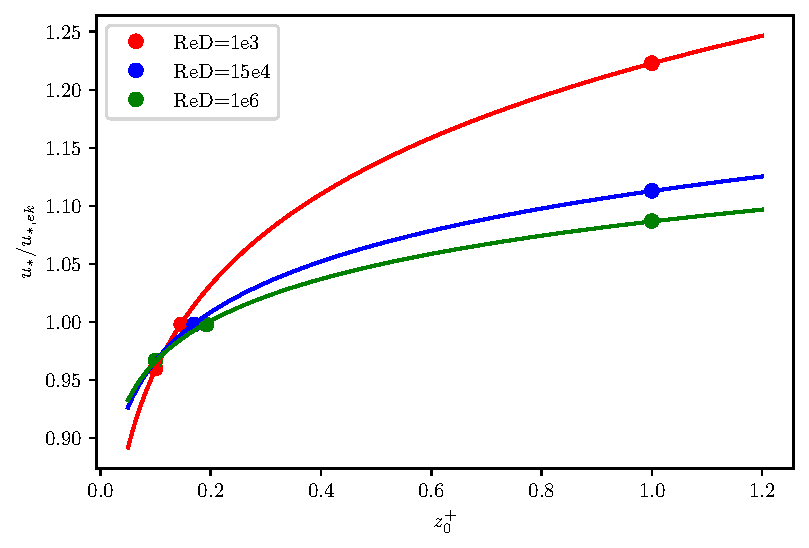
\includegraphics[width=0.45\textwidth]{figures/3Re_ust_z0p}
	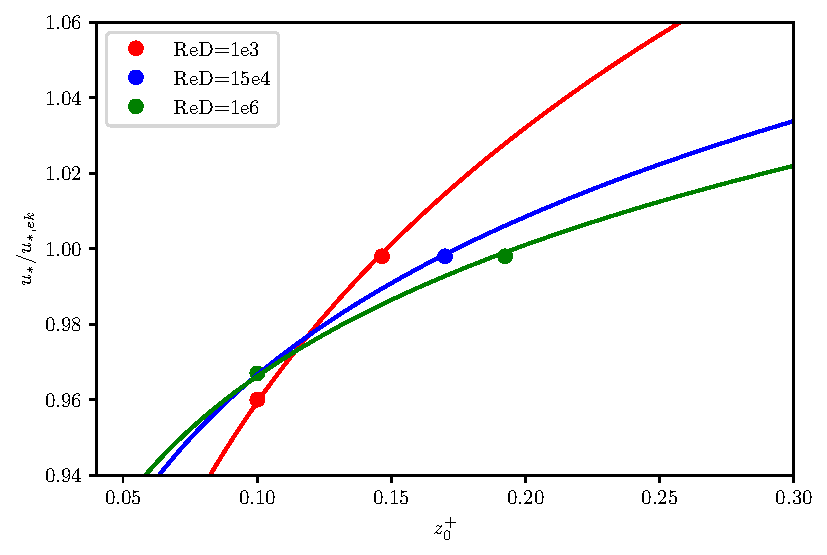
\includegraphics[width=0.45\textwidth]{figures/3Re_ust_z0p_detail}}
  \caption{The friction velocity as function of the roughness length with fit}
  \label{ust_z0p}
\end{figure}

The choice of $z_0$ and the turbulent flow (driven by the geostrophic wind $G$) determine the magnitude of $u_\star$ in a non trivial way. As will be demonstrated below, the choice of $z_0=0.1$ does not lead to the expected value of $u_\star$ predicted by Spalart. To reproduce the predicted $u_{\star pred}$, a sensitivity study was performed whose results are shown in fig. \ref{ust_z0p}. A variation of $z_0^+$ showed that the resulting $u_\star$ follow a power law $u_\star/u_{\star pred} = a(z^+_0)^m.$ In order to get the expected friction velocity, $z_0^+$ had to be 0.149, 0.174, and 0.196 for the cases Re1, Re2, and Re3, respectively. As these are the values for Reynolds numbers that differ by three orders of magnitude, this is only a slight dependence on the Reynolds number

\section{Results}

The theoretical profiles of both horizontal velocity components as well as corresponding LES solutions for all three Reynolds numbers are shown in fig. \ref{profiles_allred}. At first sight, the similar form of the profiles for all Reynolds numbers is apparent. In the viscous sublayer, the shear-aligned component increases linearly up to the buffer layer around $z^+\approx19$, where it (übergehen) slowly into the logarithmic layer. There the U-component increases logarithmically up to the supergeostrophic maximum and above decreases to its geostrophic value. The V-component plays nearly no role up to the middle of the logarithmic layer, where the transition to the Ekman layer takes place ($z^-\approx0.3-120/Re_D$). In inner scaling, the V-component of all Reynolds numbers is very similar, while the growth of the U-component leads to a smaller angle $\alpha$ for higher Reynolds numbers. In outer scaling, the profiles  of the shear-aligned velocity deficit collapse in the upper part of the boundary layer and the profiles of the V-component's velocity deficit collapse for the whole boundary layer.

The length of the profiles from the LES is identical for all Reynolds numbers. This is due to the fact that for all simulations, the ratio between boundary layer height and grid size is similar, which leads to similar lengths from the first grid point to the boundary layer top in a logarithmic plot.

\begin{figure}
  \centerline{
	\includegraphics[width=0.385\textwidth]{figures/uv_p_AllReD}
	\includegraphics[width=0.4\textwidth]{figures/uv_def_AllReD}
}
  \caption{Left: shear-aligned profiles in outer scaling. Right: shear-aligned velocity deficit in inner scaling}
  \label{profiles_allred}
\end{figure}


\todo{Show dependence of the profiles on the domain size.}

The (expression?) $\kappa = d\log(z^+)/dU^+$ is quite sensitive to the resolution as well as to the domain size.

\todo{Rating of the resolution as Jiang and Sullivan: value of $\kappa$, $z_{0,pr}$ estimated from profile vs. $z_0$, $\Delta W_{10}$}

Estimation of $\kappa$: maximum height: where the value of $\kappa = d\log(z^+)/dU^+$ of the theoretical profile deviates by more than 2\% of the used value $\kappa = 0.416$. minimum height: seventh grid point

\begin{table*}
	\centering
	\caption{Simulation results}
		\begin{tabular}{lccccc}
		  Name & $\kappa_{LES}$ & $z_{0,LES}/z_0$ & $\delta_{95}/\delta$ & $u_\star/u_{\star,dl}$ & $\alpha/\alpha_{dl}$ [$^\circ$] \\ \hline
			Re1\_150 & 0.449 & 0.36 & 0.58 & 1.00 & 0.91  \\
			Re1\_150\_dyn & 0.417 & 0.88 & 0.58 & 1.03 & 0.89 \\
			Re1\_100 & 0.485 & 0.18 & 0.61 & 1.00 & 0.89 \\
			Re1\_50 & - & - & 0.70 & 1.00 & 0.86 \\ \hline
			Re2\_150 & 0.464 & 0.09 & 0.59 & 1.00 & 0.92 \\
			Re2\_100 & 0.507 & 0.18 & 0.62 & 1.00 & 0.86 \\
			Re2\_50 & - & - & 0.73 & 1.00 & 0.85 \\ \hline
			Re2\_150\_a & 0.458 & 0.12 & 0.60 & 1.00 & 0.88 \\
			Re2\_150\_b & 0.460 & 0.11 & 0.59 & 1.00 & 0.86 \\
			Re2\_150\_c & 0.467 & 0.08 & 0.56 & 1.00 & 0.96 \\
			Re2\_150\_d & 0.477 & 0.06 & 0.57 & 1.00 & 0.97 \\ \hline
			Re2\_150\_dyn & 0.443 & 0.28 & 0.58 & 1.01 & 0.91 \\
			Re2\_50\_dyn & - & - & 0.7 & 1.01 & 0.81 \\ \hline
			Re3\_150 & 0.477 & 0.03 & 0.58 & 1.00 & 0.94 \\
			Re3\_150\_dyn & 0.453 & 0.12 & 0.62 & 1.01 & 0.86 \\
			Re3\_100 & 0.514 & 0.01 & 0.63 & 1.00 & 0.88 \\
			Re3\_50 & - & - & 0.72 & 1.00 & 0.85 \\
		\end{tabular}
	\label{simulation_results}
\end{table*}

The turbulent structures in boundary layers of high Reynolds numbers extend over a large range of scales. For the description of their vertical mean profiles, inner units ($z^+ = zu_*/\nu$, $U^+=U/u_*$) and outer units ($z^-=z/\delta$, $U^-=U/G$) are used. At the lower boundary, the x-axis of the inner units is aligned with the shear stress, whereas the x-axis of the outer units is aligned with the geostrophic wind. The angle between both axes is called $\alpha$.

A principal idea behind LES is to neglect the small scales of the flow and resolve only the large eddies, which carry most of the turbulent kinetic energy. Hence, the viscous sublayer and the buffer layer are not resolved by LES and cannot be compared. The first grid point of an LES usually lies inside of the logarithmic region of the boundary layer. Furthermore, the flow is usually underresolved in the lower layers of an LES, since near the bottom, the vertical component is massively restricted by the non-permeability of the wall.

$\delta_{95}$: height where the turbulent stress decreased to 5\% of its surface value. \todo{put $\delta_{95}/\delta$ in table. Which of both do we call boundary layer height?}

\begin{figure}
  \centerline{
	\includegraphics[width=0.3\textwidth]{figures/alt_uv_p_Re1a}
	\includegraphics[width=0.3\textwidth]{figures/alt_uv_p_Re2}
	\includegraphics[width=0.3\textwidth]{figures/alt_uv_p_Re3}
}
  \caption{Shear-aligned profiles in inner scaling}
  \label{3Re_uv_p}
\end{figure}


\subsection{Logarithmic layer stream-wise velocity}

\todo{include $50<z^+<0.15Re_\tau$, while $z^-=z^+Re_\tau$}

Figure \ref{3Re_kappa} shows $\kappa = z^+\partial U^+/\partial z^+$, which is constant in the logarithmic layer. The theoretical profile shows a constant $\kappa$ up to $z^-\approx0.1$ for the case Re1 and up to $z^-\approx0.15$ for the cases Re2 and Re3 \todo{The logarithmic layer already begins to feel the outer layer}. All cases have in common that an increase in resolution leads to a profile much closer to the theoretical curve.

A typical feature of LES is the log-layer mismatch of the first grid points above the bottom, comprehensively discussed by \cite{brasseur2010designing}. According to \cite{maronga2020improved}, mean profiles follow MOST at height levels starting from the seventh grid above the surface. \todo{\citep{jiang2018large} identify an SGS-buffer layer which starts at ...} \todo{define maximum deviation (in percent) from $\kappa$ to define the height of the (nearly) purely logarithmic region. Between the seventh grid point and this height, $\kappa$ of the LES is determined.}

\begin{figure}
  \centerline{
	\includegraphics[width=0.3\textwidth]{figures/kappa_Re1a}
	\includegraphics[width=0.3\textwidth]{figures/kappa_Re2}
	\includegraphics[width=0.3\textwidth]{figures/kappa_Re3}
}
  \caption{$\kappa$ in the logarithmic region and above for different Reynolds numbers and resolutions}
  \label{3Re_kappa}
\end{figure}

An obvious feature of the low Reynolds number case is that the viscous sublayer represents a notable share of the boundary layer, while this layer is hardly visible for the high Reynolds number cases.

A Reynolds number of $Re_D = 1\,600$ is a very unusual Reynolds number for an LES. The first grid point of the LES lies at $\Delta/2$ and should lie in the logarithmic region of the boundary layer (citation?). For the finer resolved simulations of the low Reynolds number, the first grid point lies well in the buffer layer or even in the viscous sublayer. That means that the simulation results of this point are unlikely to produce reasonable results since an LES does not comprehend the physics needed to describe the behavior of the flow in this region.

The transition from buffer layer to logarithmic layer lies around $z^+=19$. The first grid point of the simulation \textit{Re1} lies at $z^+=14$ for the 20\,cm resolution and at $z^+=10$ for the 14\,cm resolution.

The finest resolution ReX\_150 resolves well the boundary layer in agreement with the findings of Wurps2019 where the neutral simulation was well resolved with more than 100 grid levels inside of the boundary layer $\delta_95$. The ratio $\delta_95/\delta$ is roughly $2/3$ (slightly decreasing with Reynolds number). Hence, 150 grid levels within $\delta$ mean around 100 grid levels within $\delta_{95}$. 

\begin{figure}
  \centerline{
	\includegraphics[width=0.3\textwidth]{figures/alt_uv_def_Re1a}
	\includegraphics[width=0.3\textwidth]{figures/alt_uv_def_Re2}
	\includegraphics[width=0.3\textwidth]{figures/alt_uv_def_Re3}
}
  \caption{Shear-aligned velocity deficit}
  \label{3Re_uv_def}
\end{figure}


\subsection{Logarithmic layer span-wise velocity}

Figure \ref{v-comp_log}
\begin{figure}
  \centerline{
	\includegraphics[width=0.3\textwidth]{figures/v-comp_log_Re1a}
	\includegraphics[width=0.3\textwidth]{figures/v-comp_log_Re2}
	\includegraphics[width=0.3\textwidth]{figures/v-comp_log_Re3}
}
  \caption{Shear-aligned velocity deficit of the v-component in the logarithmic layer}
  \label{v-comp_log}
\end{figure}

\subsection{Ekman layer}


\begin{figure}
  \centerline{
	\includegraphics[width=0.32\textwidth]{figures/alt_alpha_zm_Re1a}
	\includegraphics[width=0.3\textwidth]{figures/alt_alpha_zm_Re2}
	\includegraphics[width=0.3\textwidth]{figures/alt_alpha_zm_Re3}
}
  \caption{Direction of the mean flow with respect to the geostrophic wind. }
  \label{3Re_alpha}
\end{figure}

Hodograph: in reality (or DNS), the wind profile shows only a very little change of wind direction near the bottom, whereas LES starts veering from the first grid point on.

For the case Re1, the curves for all resolutions fall quite well onto the theoretical hodograph. For the cases Re2 and Re3, the hodographs clearly show that the veering is underestimated by the LES.

There is a clear tendency that finer resolutions lead to a bigger $\alpha$ which is strongest for case Re3. Nevertheless, the predicted $\alpha$ is reached by non of the LES.

The adaption of the theoretical curve by using the $\alpha$ from the fines LES seems to be beneficial only for high Reynolds numbers. $\alpha$ is defined as the direction of the wind at the bottom while in LES we only have the direction of the wind at the first grid point: further veering below the first grid point is not taken into account. For high Reynolds numbers, the direction of the flow stays almost constant for a much wider part of the boundary layer (around 1\% for Re2 and Re3), while for lower Reynolds number, the direction changes significantly much earlier (around 0.1\% for Re1). The total $\alpha$ predicted by the theoretical profile (and the DNS) is $16.8^\circ$ and the $\alpha$ of the LES with finest resolution of case Re1 is $15.3^\circ$. Despite this considerable difference, the curves match quite well and LES reproduces the correct course of wind directions at all heights above the first grid point.

\begin{figure}
  \centerline{
	\includegraphics[width=0.3\textwidth]{figures/alt_hodograph_Re1a}
	\includegraphics[width=0.3\textwidth]{figures/alt_hodograph_Re2}
	\includegraphics[width=0.3\textwidth]{figures/alt_hodograph_Re3}
}
  \caption{Geostrophy aligned hodograph}
  \label{3Re_hodograph}
\end{figure}

Limits of coarse resolution - where is the MOST-Point in Hodograph?

Vergleich SGS-Modelle

As stated before, eq. \ref{drag} is very well validated for the range $400<Re_D<1\,600$ \citep{ansorge2014global}. For Reynolds numbers like $Re_D=1.5\cdot10^5$ or even $Re_D=10^6$, there exist neither DNS nor experimental data. Hence, the solutions of eq. \ref{drag} are not to be taken as certainly correct and one might assume that the LES solution is not definitively incorrect. This being said, the theoretical profiles are recalculated with the values of $u_\star$ and $\alpha$ from the LES solution. \todo{$u_\star$ genau messbar, G nicht. Trotzdem Spalart verlässlich? Integrale? Herleitung angucken. Vielleicht ist Re für die LES anders? $\delta/z_0$ Indeed, \cite{jiang2018large} use $G$, $f$ and $z_0$ as input parameters -- and these \textit{are} the input parameters for an LES. Why are we adjusting $z_0$ to get the $u_\star$ predicted by \cite{spalart1989theoretical}?} Simulations of \cite{jiang2018large} are not the same as ours, since their choice of $z_0$ is a real roughness length and not just caused by the viscosity and a flat plate. Their roughness lengths are so high that the resulting viscosity would have to be considered in the Navier-Stokes equations.


\section{Discussion and Conclusions}

Interesting comparison between DNS and LES

Overall: good fit between theoretical profile and LES

Resolution of LES matters a lot

Helpful for rating LES profile: height where profile should deviate from logarithmic shape.

Theoretical profiles provide a very detailed benchmark for all aspects of the flow. A very good hit of the hodograph might coincide with a poor curve for $\kappa$.

\bibliographystyle{plainnat}
\bibliography{papers.bib}


\end{document}
